\documentclass[border=2pt]{standalone}
\usepackage{newtxtext,newtxmath}
\usepackage{tikz,pgfplots,amsmath}
\usetikzlibrary{arrows.meta,positioning,calc,shapes.geometric}
\pgfplotsset{compat=1.18}
\definecolor{navy}{HTML}{24465E}
\definecolor{teal}{HTML}{327F83}
\definecolor{coral}{HTML}{BF594C}
\definecolor{ochre}{HTML}{AC7A28}
\definecolor{slate}{HTML}{67737D}
\definecolor{mist}{HTML}{E4E9EC}
\definecolor{pale}{HTML}{F4F7F8}
\definecolor{wine}{HTML}{885878}
\definecolor{lightteal}{HTML}{E3F0EF}
\tikzset{every node/.style={font=\sffamily\fontsize{8}{9.5}\selectfont},
 block/.style={draw=slate!65,fill=pale,rounded corners=1.5pt,inner sep=5pt,align=center},
 link/.style={-{Latex[length=1.8mm,width=1.15mm]},draw=slate,line width=.65pt}}
\pgfplotsset{every axis/.append style={
 font=\sffamily\fontsize{8}{9.5}\selectfont,
 tick label style={font=\sffamily\fontsize{7}{8.3}\selectfont,/pgf/number format/fixed,/pgf/number format/precision=3},
 label style={font=\sffamily\fontsize{8}{9.5}\selectfont},
 axis line style={slate!70,line width=.45pt},tick style={slate!70},
 grid style={mist,line width=.35pt},
 legend style={font=\sffamily\fontsize{7}{8.2}\selectfont,draw=none,fill=white,cells={anchor=west}},
 scaled ticks=false,clip=true,mark size=1.6pt}}

\begin{document}
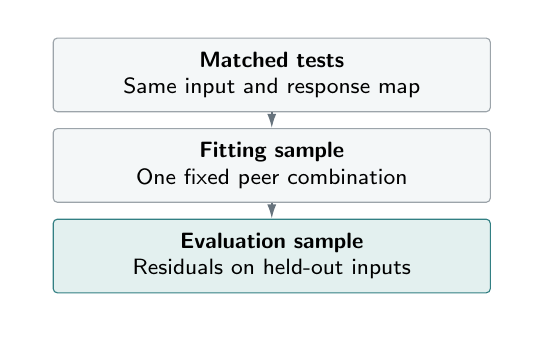
\begin{tikzpicture}

\path[use as bounding box] (-3.1,-.65) rectangle (3.1,3.05);
\node[block,text width=5.2cm,minimum height=.65cm] (q) at (0,2.45)
 {\textbf{Matched tests}\\Same input and response map};
\node[block,text width=5.2cm,minimum height=.65cm] (f) at (0,1.30)
 {\textbf{Fitting sample}\\One fixed peer combination};
\node[block,text width=5.2cm,minimum height=.65cm,fill=lightteal,draw=teal] (e) at (0,.15)
 {\textbf{Evaluation sample}\\Residuals on held-out inputs};
\draw[link] (q.south)--(f.north);
\draw[link] (f.south)--(e.north);

\end{tikzpicture}
\end{document}
